\documentclass[11pt]{article}
\usepackage{cs65f12}
\usepackage{times}
\usepackage{latexsym}
\usepackage{enumerate}
\usepackage{graphicx}
\setlength\titlebox{6.5cm}    % Expanding the titlebox

\title{Word Segmentation in Morphological Analysis}

\author{Steve Dini\\
  Computer Science Department\\
  Swarthmore College\\
  {\tt sdini1@cs.swarthmore.edu}  
  \And                            %omit if
  Emanuel Schorsch\\                 %there isn't
  Computer Science Department\\
  Swarthmore College\\
  {\tt eschors1@swarthmore.edu}}

\date{}

\begin{document}
\maketitle
\begin{abstract}
This paper provides an overview of various methods for segmenting words and 
an analyis of how each of the methods performs in terms of precision
and recall. We segmented words using successor and predecessor counts as well
as various modifications to these methods including successor cutoff. 
Towards the end we discuss an attempt at implementing Dejean's 
algorithm, some modifications, shortcomings with the implementation
as well as discussion of possible solutions to the said shortcomings. We then
tested our implementations on a list of 1000 'properly' segmented English words.
  
\end{abstract}

\section{Introduction}

Morphological analysis, which deals with the segmentation of words, is one of 
the most fundamental areas of Natural Language Processing. There has been a 
myriad of methods and algorithms that have been implemented to make this 
process as accurate and efficient as possible ~\cite{hafer1974-word}. The importance of word 
segmentation in morphological analysis can be mostly seen in
morphologically complex languages in which the automatic identification of
morphemes is an involved process. Identifying the morphemes in agglutinative
languages like German, though easy to the human linguist, is very hard for a 
machine to do.\\
However, it is not always clear what the correct segmentation is, even to
human linguists. Prefixes, suffixes and infixes must all be seperated. Yet
often due to changed spellings the suffix can be interpreted as any of a 
number of different things. This potentially makes the task more challenging.
Depending on the task, as long as the segmentations are consistent it is
sufficient, even if the system is not performing with perfect accuracy on some
gold standard segmentation.
Another motivation for the development of word segmentation is the need to 
identify root forms of words and use it do processing we might have wanted to 
do using the initial word. The benefit of doing it this way is that we reduce 
the spatial breadth of our word-space. This makes storage and retrieval of 
words a more efficient process. \\
There are many more applications of identifying the stems of words including
language translation and search engines. Since the systems we are analyzing
stand independently of any task, we cannot evaluate them by their performance
on some external task. Therefore our judgment of the relative performance of
the different techniques is based mostly on the recall and precision metrics 
which are defined later. \\
The Harris~\shortcite{harris1955-phoneme} paper introduces the notion of 
successor and predecessor frequency. His segmentation is conducted mainly
using the detection of peaks among these frequencies. This concept is then
expanded on by Hafer and Weiss. They include
peak analysis and combine it with a cutoff and entropy method
~\cite{hafer1974-word}. They investigate numerous different combinations of
these methods, a few of which we have 
implemented and describe in the paper. Finally, Dejean describes a fairly
complex algorithm which is inspired by Harris's paper and focuses on
identifying a plausible set of suffixes and prefixes in the language and then
using these affixes in segmentation.
~\cite{dejean1998-morphemes}. 
\section{Methods}
\begin{figure}[h!]
  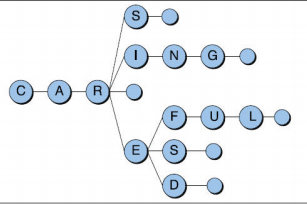
\includegraphics[width=80mm]{imgs/trie.png}
  \caption{Trie Data Structure}
\end{figure}

For our implementations,
we used a trie, which is an ordered tree data structure which is used to store
a dynamic set or associative array and is built in such a way that it easily
supports longest prefix matching when performing lookups.
The trie contained frequency counts for how many times a word fragment
had appeared in the corpus. Two tries were created, one for the words, and
another for the words reversed. This allowed us to calculate predecessor
statistics more easily. The structure of the trie allowed us to easily
calculate how many different letters ever appeared after a specified word
segment.
\begin{enumerate}[(a)] 
\item In the Predecessor Cutoff system we segmented words whenever the
  predecessor count exceeded some arbitrary cutoff. This cutoff is determined
  experimentally. Given our corpus, two reasonable cutoff values were chosen.
  Cutoff values of either 14 or 22 were found to be acceptable. The difference
  between them, and when you would use each will be discussed in the results.
\item A system which segments whenever successor frequency exceeds the cutoff
  is atrocious, since successor frequency decreases nearly monotonically from
  left to right. Therefore we investigated a combined system which used both
  predecessor and successor frequencies. The algorithm segmented words when
  both counts were above their respective cutoffs. This demonstrated
  what a more restrictive system system would look like.
\item A natural alternative to the previous system is to take the other
  approach and relax requirements. Simply taking the union of when either
  counts reached a cutoff would cut in too many places. Instead the system
  cuts whenever the sum of the counts exceeds the chosen cutoff. This allows
  high values of either predecessor or successor frequency to trigger a 
  segmentation.
\item The middle approach between the above two procedures is to require
  that one value be high and the other at least be moderate. The specific
  implementation was that a cut was triggered when the word fragment had been
  seen before as a complete word in the corpus and the predecessor frequency
  was at least 4. Additionally a segmentation could also occur if predecessor
  frequency was greater than 18 and successor frequency was at least 2.
\item A simple system to implement is one which only cuts when the word
  fragment has been seen as a complete word in the corpus. This obviously
  works better with a larger corpus. Given the high frequency of small 
  independent words which are not actually stems it is necessary to only
  trigger the segmentation if the fragment is 4 or more letters. This fragment
  length was experimentally chosen as it made our precision the greatest.
\item The next two algorithms utilize the concept of a peak or plateau.
  A peak or plateau is if the count is greater than or equal to the counts to
  the immediate left and right. The scope is therefore very local, so that
  a peak can occur even among other low counts. The first system which uses
  this just segments whenever there is a peak in the successor frequencies.
\item Naturally the above was also investigated for solely predecessor
  frequencies. These algorithms have the disadvantage of being unable
  to distinguish peaks once counts get very low. Further when the counts are
  very high it is easy for noisy peaks to arise that don't represent true
  salient features of the word.
\item A more interesting system is one that requires a peak in both 
  successor and predecessor frequencies in order to segment at a point.
  This obviously reduces the noise of the system, at the cost of being
  less sensitive.
\item In an effort to be less restrictive the next system requires a peak
  in the sum of the predecessor and successor frequences. At each index
  the successor and predecessor frequency are summed. The new counts that
  result are fed into the peak detection algorithm.
\end{enumerate}

\section{Dejean's Algorithm}
In addition to the algorithms stated above, we also attempted to implement the
algorithm proposed by Dejean ~\cite{dejean1998-morphemes} The algorithm provides for unsupervised
learning in which you have no prior knowledge about the corpus you are working
with. The mechanics of the algorithm are such that you begin by looking for the
most frequent morphemes in your corpus based on the successor frequencies 
method ~\cite{hafer1974-word}.  Instead of using a successor cutoff as originally proposed,
we had our implementation use successor peaks because the cutoff threshold 
appeared to be specific to each corpus. Further the cutoff threshold in one corpus
did not always give the best results in another corpus. Even though the
algorithm suggested keeping entries with a frequence greater than 100 (again
corpus dependent), we decided to keep anything with a frequence greater than 2
on the premise that this set of morphemes was small enough to manage.
It turns out that after this initial pass through the corpus, the set of 
morphemes we had was entirely composed of prefixes and suffixes as can be seen 
in figure 1.\\
\begin{figure}[h!]
  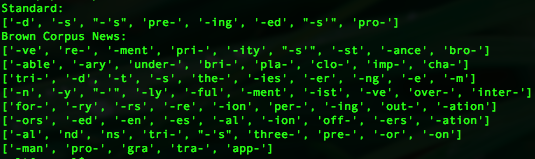
\includegraphics[width=100mm]{imgs/affixes.png}
  \caption{List of created morphemes}
\end{figure}
Once these morphemes are discovered, another pass through the 
corpus is performed in which case more affixes can be discovered. The rationale
behind this second pass is that if a root can be identified that exists as a 
word when some of the affixes in our set are attached to it, then any other
affix attached to that root not in our set should be added to the set. Dejean
suggests that we should add these new morphemes only if half of the affixes 
that complete the root already exist in our morphemes set. We felt this was
corpus-specific and our blind implementation of this suggestion yielded
terrible results (precision $< 0.01$). In light of this, we made a 
slight modification and only added if at least 3 of the possible affixes
already existed in our set. This proved to be fruitful as we were
now in a position to build the entire list of reasonable affixes from the 
corpus. The threshold we used was not without its pitfalls: There were some 
words that were clearly not affixes that were identified as affixes. However, 
this was less than $5\%$ of the entire set of acceptable results and so did not
significantly alter our results.\\
The next stage in this algorithm involved actually segmenting the words using
the set of acceptable affixes that we built from the last stage. In cases where
more than one affix matched the beginning or end of a word, we went ahead and 
picked the longest match as was suggsted in the algorithm. It was also
interesting to note that on average we were only able to find 1 or 2 more 
affixes, an observation we largely attribute to the corpus. Either the corpus
was not diverse enough to include multiple forms of the same root or it
was just the case that the corpus was so large that we had effectively explored
all the possible affixes that could be attached to the stem. At this point, 
everything appeared to be on the right path. One more piece of the puzzle and
our implementation would be complete.\\
It turns out the last piece of the puzzle was more involved than
we anticipated. Dejean argues that inconsistencies with the segmentation 
results are to be expected. This is primarily because since we picked the 
longest matching affix in the last step, we would need to resegment those 
affixes when necessary using contextual information. This can be achieved by
building bigrams of morphemes in the last stage and then using contextual
information from that to perform further segmentation. The only examples
provided in the paper include the sequence des Hauses in German in which 
further segmentation yields des Haus-es. The interesting thing to note with
those examples is that the languages referenced (French and German) allow
for quantititave articles (le vs les) that supply this contextual information.
This is not the case in a language like English and as such were not able to
implement this last piece of the puzzle and perhaps that was responsible for
the unusually low results we obtained using this method.

\section{Results}
Precision is a metric that is used to define the percentage of retreived 
instances that are relevant while recall is that percentage of relevant 
instances that are retreived. Precision measures
how confident you are that any given segmentation is correct. Recall measures
how many of the correct segmentations you are detecting. It is simple to get
either perfect precision or perfect recall: precision, by only segmenting one
word which you know, and recall, by segmenting after every single letter.
Therefore the optimal results are for both precision and recall to increase,
and be sufficiently high.\\
Table 1 gives a representation of the results we obtained after running our
algorithms on the provided gold standard of 1000 segmented words. Table 2 gives
the same results, the only difference being the fact that we ran our 
algorithm on the gold standard of 50 words that we created and manually 
segmented. We acknowledge the fact that there a qualitative differences in
the results between the 2 runs, and the only plausible explanation is that
the sizes of the test sets are off by an order of magnitude hence this might
put a strain on the level of morphological diversity that can be achieved.\\
\begin{table*}
\centering
\begin{tabular}{ l  c || r }
  Method & Precision & Recall \\
    (a) Successor and predecessor $\leq$ cutoff & 48.122 & 11.252\\
    (b) Dejean's Algorithm & 29.51 & 21.84\\
    (c) Reverse Cutoff (k=14) & 55.046 & 38.308\\
    (d) Reverse Cutoff (k=22) & 71.96 & 29.289 \\
    (e) Sum Cutoff (k=22) & 71.317 & 29.369 \\
    (f) Duo Peaks         & 78.26 & 8.619 \\
    (g) Sum Peaks         & 58.219 & 47.486 \\
    (h) Negative Frequency &76.657 & 23.064 \\
\end{tabular}
\caption{Segmentation Results on Rich's Gold Standard}
\label{tab:table1}
\end{table*}

\begin{table*}
\centering
\begin{tabular}{ l  c || r }
  Method & Precision & Recall \\
    (a) Successor and predecessor $\leq$ cutoff & 58.823 & 15.625\\
    (b) Reverse Cutoff (k=14) & 17.073 & 21.212\\
    (c) Reverse Cutoff (k=22) & 11.764 & 9.09 \\
    (d) Sum Cutoff (k=22) & 62.5 & 24.590 \\
    (e) Duo Peaks         & 85.714 & 9.090 \\
    (f) Sum Peaks         & 61.224 & 50 \\
    (g) Negative Frequency & 80 & 24 \\
\end{tabular}
\caption{Segmentation Results on Generated Gold Standard}
\label{tab:table2}
\end{table*}

\begin{table}
\centering
\begin{tabular}{ l  c  r }
  Corpus & Precision & Recall \\
    (a) News corpus & 8.84 & 3.99 \\
    (b) Gold Standard & 29.51 & 21.84\\
\end{tabular}
\caption{Segmentation results using Dejean}
\label{tab:table3}
\end{table}

\begin{table}
\centering
\begin{tabular}{ l  c  r }
  Corpus & Precision & Recall \\
    (a) News corpus & 8.84 & 3.99 \\
    (b) Gold Standard & 29.51 & 21.84\\
\end{tabular}
\caption{Segmentation results using Dejean}
\label{tab:table3}
\end{table}


\section{Analysis}
Our algorithms did not reach the levels of performance seen in the Hafer and
Weiss paper. This could very well be because Hafer and Weiss trained and
tested on easier corpora. When we retested on a handcrafted gold standard
our performance dramatically improved across the board. This was due to our
choice of 'normal' words, which didn't have many abnormal segmentations.

One of the most common errors we made with an algorithm such as the sum peak
segmenter was to not segment off a plural 's'. This is strange as the
algorithm was able to segmented off 'ed' and 'ing'. This may have arose due
to it being difficult to have a sum peak after the very first letter. This is
because predecessor frequency will usually be relatively high for the first 
two letters. Obviously when we segmented words whenever they appeared as
complete words in the corpus we had much better success with such endings.
This is because a plural 's' which should be segmented almost always comes after
a real word, which appears in the text by its own. 

\section{Future Work}
A handicap we discovered with Dejean's Algorithm is that the last pass really
depends on the morpheme bigrams having a contextual relationship. This can
only be generated in languages like French and German that have the concept
of quantitative determiners and articles (le vs les). In English this is not
the case, and one way we were thinking of embedding this contextual
information was to use part-of-speech tagging. Although this appears to violate
the notion of the method being unsupervised, we believe it will greatly 
improve the quality of the segmentation and get precision and recall values 
that have been observed when performing segmentation in languages like French
and German.

One natural extension of some of the poor segmentations that were occuring
towards the ends and beginning of words is to combine two or more algorithms.
For instance if we combined sum peak analysis with negative frequency we might
be able to identify prefixes and suffixes better. This is because the
successor and predecessor frequencies usually decrease monotonically, so by
the ends and beginnings of words the algorithm is more sensitive to noise.

Another intriguing idea we had is to segment words and then feed what appears
to be the segmented root back into the negative frequency algorithm. This has
the advantage of avoiding the highly inneficient method of check every
possible substring of every word to see if any word in the dictionary appears.
Many words which have both prefixes and suffixes could then be better
segmented if the prefix was cut off and then the substring appearing after
the prefix could be located in the dictionary. This would allow the suffix to
be identified as well. We saw in our results that negative frequency is very
precise, so this would only improve our results.

\section{Conclusions}
Our best algorithms did not perform horribly, producing many reasonable
segmentations in both the thousand word gold standard, and our handcrafted
one. There was not an insignificant number of arbitrary segmentations
which appeared to have no linguistic reason. However, many of the segmentations
which were marked incorrect were actually quite reasonable and were simply
a matter of interpretation. In general our algorithms erred on the side of 
precision, which is useful in many applications in which this kind of 
segmentation would be used.

\bibliographystyle{cs65f12}
\bibliography{cs65f12}

\end{document}
